This section describes the results of applying the algorithm discussed
in \Autoref{sec:algorithm} to the experiment described in
\Autoref{sec:experiments:setup}.  We briefly summarize the results.
The algorithm identified a highly-ranked cause that would be useful to a programmer
for seven of the nine bugs.  For the two other bugs,
one (bug \#7) occurred in our experiment but never caused
the program to crash or produce incorrect output; the other (bug \#8) was never
triggered at all.  There is no way our algorithm can find causes of bugs that do not
occur, but recall that part of our purpose in sampling user executions
is to get an accurate picture of the most important bugs. It is consistent with
this goal that if a bug never causes a problem, it is not only not worth fixing,
it is not even worth reporting.

A surprise in the experiment was that we found a bug \#10; the results
showed us a previously undiscovered bug in \moss.

We performed 31,996 random runs of \moss.  Of these, 123 runs were
discarded because they produced no report (see
\Autoref{sec:experiments:setup}), giving us 31,873 runs to work with.

For this experiment we enabled all three instrumentation strategies
described in \Autoref{sec:background}:

\begin{description}
\item[branches:] 2085 instrumentation sites.  Each site has two
  counters and yields two predicates, for 4170 branch predicates.

\item[returns:] 494 instrumentation sites.  Each site has three
  counters and yields six predicates, for 2964 return predicates.

\item[scalar-pairs:] 32,644 instrumentation sites.  Each site has
  three counters and yields six predicates, for 195,864 scalar-pair
  predicates.
\end{description}

Thus, the input to our analysis is 31,873 feedback reports, each of
which records the status of over 200,000 predicates.  The reader may
wonder whether it is practical to actually generate a report on
200,000 predicates on a client machine and then upload it to a central
server for analysis.  The answer is definitely yes.  First, recall
that the predicates are synthesized from about half as many counters.
The counters are mostly zeroes and so compress extremely well,
resulting in uploaded files in the range of 10-50K.

The sampling rate for all runs in this experiment was \nicefrac{1}{1};
i.e., we sampled every predicate every time it was reached.  An
offline downsampling program lets us generate sparser samples from this
full data; thus, we were able to use the same set of runs to test the
effect of different sampling rates on the results.

The time to run our algorithm on all the runs is about seven minutes on
a fast machine.
At \nicefrac{1}{100} sampling, step (1) of our analysis algorithm eliminates about 99\% of
all branch and return predicates, and about 96\% of the scalar-pair
predicates.  We retain only
\begin{itemize}
\item 51 branch predicates;

\item 16 return predicates;

\item 8672 scalar-pair predicates.
\end{itemize}

Clearly the scalar-pairs list is still too long after step (1) to
process by hand, even if we only look at the highly-ranked predicates.
We often noticed that in the scalar-pairs report many closely related
predicates are reported for the same line number.  For our experiment,
we simply reported only one predicate per line, and then browsed the
entire list of other predicates on that line if it appeared
interesting.\footnote{There are principled ways to choose the
representative predicate for a line, but we didn't need anything
better than an arbitrary choice for this experiment.}  Retaining one
predicate per line gives us a much shorter list of 186 lines to
examine (i.e., only 186 distinct lines in the program had predicates
with positive $\increase(\ldots)$ scores).

\subsection{The Bugs}

We examined the reports generated with \nicefrac{1}{100} downsampled data.
The branches report has 4 predicates with a 1.0 crash rating:
%%
\begin{small}
\begin{verbatim}
0.94 Inc, 1.00 Cr, 0.06 Co, process_file_pass2 line 5523
0.80 Inc, 1.00 Cr, 0.20 Co, handle_options line 5742
0.80 Inc, 1.00 Cr, 0.20 Co, string2lang line 4366
0.78 Inc, 1.00 Cr, 0.22 Co, handle_options line 5789
\end{verbatim}
\end{small}

Each line of a report lists the increase, crash, and context scores of
a predicate, as well as the function name and line number where it
occurs.  We have dropped some fields of the report (such as the text
of the predicate itself and the number of failing and successful runs
in which the predicate is observed) to avoid clutter.

The first predicate listed does not immediately suggest what the cause
of failure might be. By looking at the failure log, we see that this predicate
is highly correlated with a subset of the runs in which bug \#1 is
triggered; an engineer with a deep understanding of how \moss\ works
might be able to figure out the bug from this predicate alone.
The next three predicates are obvious ``hits.''  The second predicate
tests whether comment matching should be turned on, and if it is turned on the program is
guaranteed to fail. This is a much more obvious cause for bug \#1, and the predicate points directly
to the fact that something is wrong in the comment matching
code.\footnote{Recall that bug \#1 is non-deterministic; why then is
  the crash score 1.0?
The discrepancy is the result of sampling error.  In the full data set
(with \nicefrac{1}{1} sampling) the crash measure for this predicate is indeed
only 0.88.}
The
next predicate marks the test in the code that decides whether \moss\ is analyzing Lisp
programs; the crash score of 1.0 tells us that whenever a Lisp program is
processed, \moss\ crashes.  The fourth predicate
is an obvious cause of
bug \#6; it reveals that whenever the amount of memory to use is set
via a command line option, the program will crash.  (The full data set shows that bug \#6 is non-deterministic with respect to this predicate, so once again the certainty that the program will crash is the result of sampling error.)  All three of these predicates illustrate the potential of our method to
help pinpoint the root cause of a crash rather than just where the crash
happened.  Each of these predicates immediately suggests
what test case to try to reproduce the bug.

The 9th listed cause in the branches report says that whenever the
user supplies the command line option to write a database, the chance
of failure jumps to 62\% (bug \#2), and the 14th ranked cause says
that whenever a database is read the chance of failure is 55\% (bug
\#3).  All the other causes between the 5th and 21st in the branches
report are predicates that also implicate one of bugs 1, 2, 3, 5, or
6.  Below the 22nd listed cause the $\increase(\ldots)$ scores drop to
1\%; we did not examine these predicates.

The returns report is also quite interesting.  Recall that this
instrumentation scheme samples the return values of functions (whether
they are negative, positive, or zero).  The first two entries in this
report are the results of string comparisons that point directly to bug
\#5.  The third entry is the {\tt open} call in the function that writes
a database; the predicate shows that when this function returns {\tt NULL},
the program is guaranteed to crash (i.e., 1.0 crash score).  This is the
cause of bug \#2.

The fourth entry of the full data (not the \nicefrac{1}{100} downsampled data)
returns report is very interesting.  This predicate shows that one of
the file read operations in the function that loads a database can
fail, and when it does \moss\ itself fails with probability 0.64.
It turns out that \moss\ assumes that any database it reads has the
correct database file format, because it does no checking to ensure
that the read operations that actually load the database succeed.  This is a previously
unknown bug in \moss.  It is a bit surprising that this bug was detected,
because a run is only labeled a failure in our experiment if the
reference \moss\ and the buggy \moss\ differ in their outcome, and
this bug is present in both versions.  Thus, this bug could only be detected
when another one of the introduced bugs was also triggered in the same
run and caused the buggy version of \moss\ to fail in a different way.
This explains the very low $\increase(\ldots)$ score for this
predicate (the chance of failure only increases by 11\% when this bug
occurs) and why it was not observed in the \nicefrac{1}{100}
downsampled data.  With enough runs it would be observed at
any sampling rate, but the anomaly that the reference and buggy
versions of \moss\ share this bug means that, at the
\nicefrac{1}{100} sampling rate, many more runs are likely needed
than what we had for this experiment.

Bugs \#4 and \#9 have no causes in either the branches or the returns
reports, as they are not correlated with any branch nor with the
result of any function call.  In the \nicefrac{1}{100} downsampled
scalar-pairs report, there are obvious causes showing that the array
bounds have been exceeded which are ranked 26th (for bug \#4) and 52nd (for bug
\#9).  In both cases it didn't matter which predicate we chose to
represent the bug for the line identified as the cause of the bug; all
of the predicates were essentially the same.  The other
predicates ranked higher than 52nd in the scalar-pairs report are
either more obscure, but more deterministic, indicators for bug \#4 or
for one of the other five observed bugs.  Given the emphasis on
determinism in our ranking function, bug \#9 could not be listed
higher, as it is the most non-deterministic bug in our data set with a
$\crash(\ldots)$ score of 0.72.

Finally, we compared the reports generated from \nicefrac{1}{100} sampled data
with the reports generated from \nicefrac{1}{1} sampled data.  The reports were
similar, but not identical.  In particular, the ordering of the
predicates was slightly different and a few predicates with relatively
few observations or a low $\increase(\ldots)$ score --- and thus high
sensitivity to whether one or two successful or failing runs were
observed or not --- appeared on
%one list and not the other.
the \nicefrac{1}{1} list but not the \nicefrac{1}{100} sampled list.

In summary, our algorithm did a good job of producing concise reports that not
only identified the bugs, but also gave useful information about the root causes and
how to reproduce the bugs.  In addition, the algorithm identified a previously unknown
bug.

\subsection{Analysis of Predicate Elimination}

To more clearly understand how well the algorithm works,
we consider what sorts of predicates are eliminated and why.
\Autoref{tab:predelim} classifies the most common kinds of predicates
$P$ for which $\increase(P) \leq 0$.  Recall that we have
approximately 200,000 predicates for \moss.  The categories are:

\begin{itemize}
\item  A \termdef{dead} predicate is one that is not observed in any run and hence
deemed unreachable.  Nearly half the instrumented predicates are dead.

\item An \termdef{invariant} is a predicate that is observed in some run and, moreover,
is either true every time it is observed or false every time it is observed,
and is therefore presumed to be a program invariant.  More than a quarter of
the instrumented predicates are invariants.

\item An \termdef{aftermath} is a predicate that is not observed in any successful run but
is observed in some failing run, and is therefore deemed to be a secondary consequence
of a bug.  A relatively small number of predicates are aftermaths, but clearly
the impact on our reports would be large if this class of predicates were not eliminated.

\item A significant number of additional predicates are eliminated that do not fit
neatly into one of the other categories.

\end{itemize}

\begin{table}
\centering
\caption{Classification of eliminated predicates.}
\vspace{\baselineskip}
\begin{tabular}{|l|r|r|r|r|}
\hline
\multicolumn{1}{|c|}{\textbf{predicate}} &  \multicolumn{4}{c|}{\textbf{sampling rate}} \\
\cline{2-5}
\multicolumn{1}{|c|}{\textbf{category}}  &  \textbf{\nicefrac{1}{1}} & \textbf{\nicefrac{1}{10}} & \textbf{\nicefrac{1}{100}} & \textbf{\nicefrac{1}{1000}} \\
\hline
\hline
dead      &  92810 & 92810 & 92834 & 95210 \\
\hline
invariant &  56418 & 56614 & 57082 & 57034 \\
\hline
aftermath &  5666  & 5954  & 6534  & 7032 \\
\hline
other     &  38762 & 36768 & 36504 & 33023 \\
\hline
\end{tabular}
\label{tab:predelim}
\end{table}

\subsection{Effect of Sampling on Predicate Selection}

We now examine the effect of the sampling rate and the number of
program trials on step (1) of the algorithm: predicate selection.
We start with $3000$ randomly
selected trial runs, and add $3000$ random trials at a time, until we
incorporate all $31,873$ runs of our data.  We record the number of
predicates retained at each step.  This process is repeated ten times
for each sampling rate, with ten different random permutation sequences
of our data. We plot the mean and the confidence interval (one
standard deviation above and below the mean) in
\Autoref{fig:predkept-a}.  When all $31,873$ trial
runs are used, we retain $8129$ predicates when the data is not
sampled (i.e.,\ sampling rate is $\nicefrac{1}{1}$), $8807$ at sampling
rate $\nicefrac{1}{10}$, $8309$ at $\nicefrac{1}{100}$, and $8936$ at
$\nicefrac{1}{1000}$.

\begin{figure*}
  \subfigure[branches, returns, and scalar pairs]{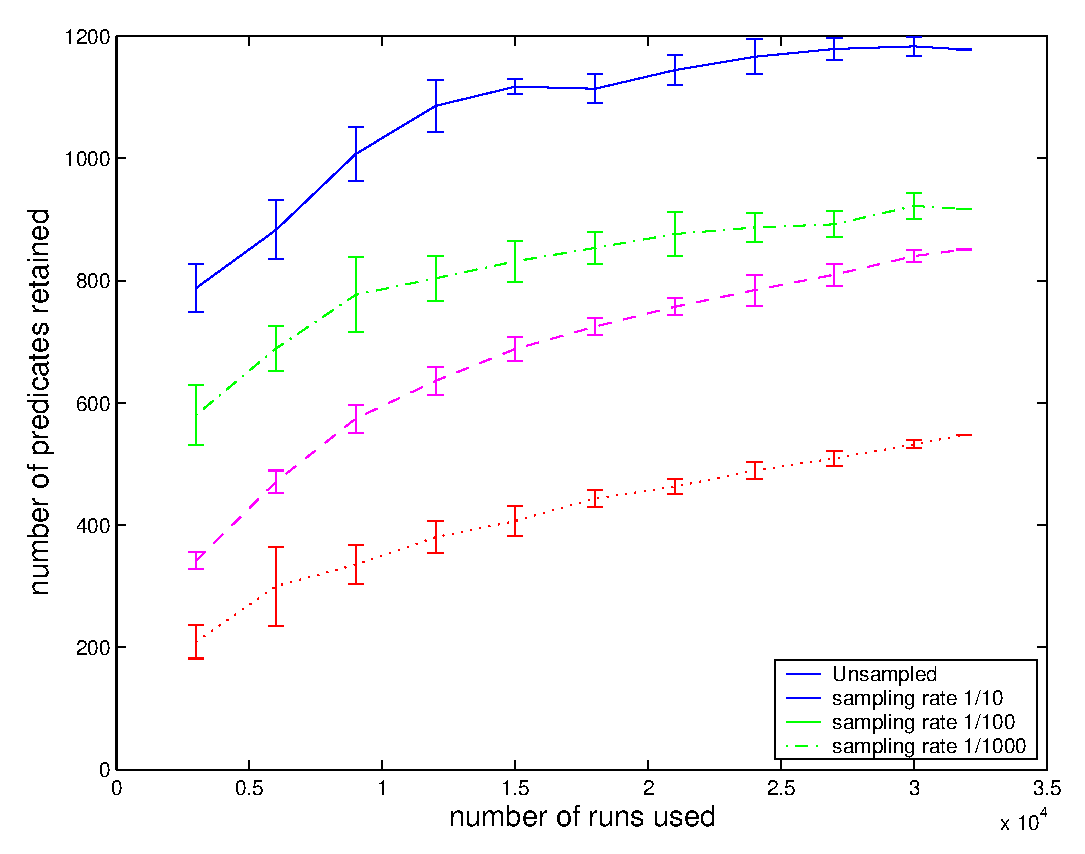
\includegraphics[width=\columnwidth]{predkept3a}\label{fig:predkept-a}}
  \hfill
  \subfigure[branches and returns only]{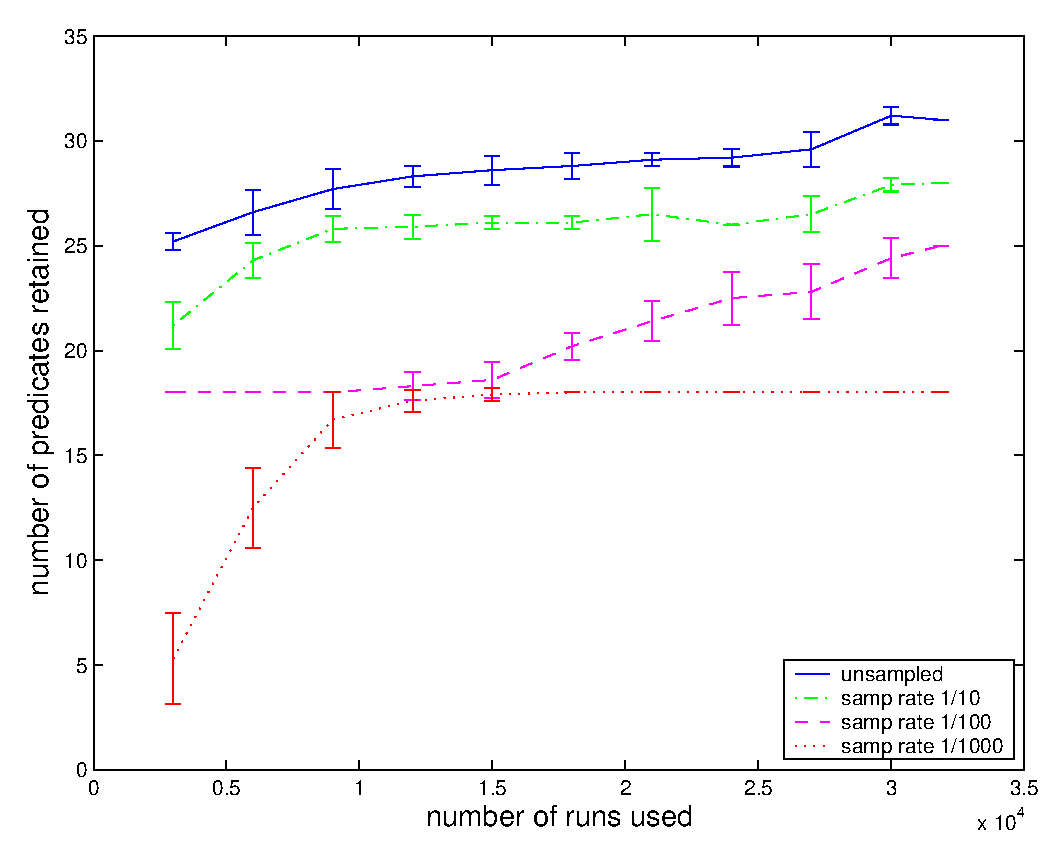
\includegraphics[width=\columnwidth]{predkept3b}\label{fig:predkept-b}}

  \caption{The effect of sampling and data size on the number of
  predicates selected.}
\end{figure*}

As is apparent from the graph, there is much larger variation in the
number of selected predicates when we use fewer trial runs.
%Using $3000$ trials, at the minimum we
%retain $7429$ predicates using unsampled data, $7654$ when sampling
%rate is $\nicefrac{1}{10}$, $7347$ at $\nicefrac{1}{100}$, and $6750$
%at $\nicefrac{1}{1000}$;
As we incorporate more examples of successful and failed \moss\ runs,
the variances decrease for all sampling rates, but the means behave
somewhat differently.  When the data is not sampled, the average
number of selected predicates stays around $8100$ for all data sizes.
Sampling adds noise to this procedure.  As we observed previously,
a moderate sampling rate tends to drive up the $\increase(\ldots)$ scores, and
thus enlarges our set of selected predicates (except when we are using
very few trial runs).

At the relatively high sampling rate of
\nicefrac{1}{10}, there are still enough samples taken at most
instrumentation sites, and there is a net increase in the number of
selected predicates.  Once the sampling rate shrinks to
\nicefrac{1}{100} and below, however, the effect of sparse
sampling sets in.  Fewer samples are taken overall on fewer predicates,
and as a result, fewer predicates have a nonzero $\increase(\ldots)$ score.
Incorporating more runs tends to alleviate the situation; at above
10,000 runs, roughly the same number of predicates are retained for
the \nicefrac{1}{100} sampled data as the complete data.  The very
sparse sampling rate of \nicefrac{1}{1000}, on the other hand,
causes much more change in the final result.  A lot more predicates
are eliminated when using fewer trials, and a lot more predicates are
retained using more trials.

Most of the volatility in the results come from the scalar-pair
predicates.  \Autoref{fig:predkept-b} shows the same graph for
only the branch and return predicates.  Here, across all data sizes,
the number of selected predicates remains roughly constant at each
sampling rate.  The complete data is still able to select the fewest
number of predicates, with \nicefrac{1}{100} sampled data following
close behind.  The \nicefrac{1}{1000} sampled data still produces a
net increase in the number of selected predicates.

%% LocalWords:  downsampling lang downsampled predelim predkept
